\documentclass[11pt,a4paper,onecolumn,oneside,notitlepage]{article}
\usepackage[utf8]{inputenc}
\usepackage[english]{babel}
\usepackage{amsmath}
\usepackage{amsfonts}
\usepackage{amssymb}
\usepackage{graphicx}
\usepackage{bbm}
\usepackage[left=2cm,right=2cm,top=2cm,bottom=2cm]{geometry}

\usepackage[backend=biber, %% Hilfsprogramm "biber" (statt "biblatex" oder "bibtex")
style=authoryear, %% Zitierstil (siehe Dokumentation)
natbib=true, %% Bereitstellen von natbib-kompatiblen Zitierkommandos
hyperref=true, %% hyperref-Paket verwenden, um Links zu erstellen
]{biblatex}
\addbibresource{paper.bib}

\author{Mokrane Yahiatene\\
	\begin{small}
		Deep Learning for Natural Language Processing -- SS21 -- Philipp Cimiano and Philipp Heinisch
	\end{small}
}
\title{SemEval-2020 Task 7: Assessing Humor in Edited
	News Headlines - Subtask 2 (Funnier)}
\begin{document}
	\maketitle
	
	\section{Introduction}
		Humor is a communicative ability resulting in laughter and joy for humans. Assessing text based humor has peaked the interest of many researchers and has been a very challenging task in the Natural Language Processing field.
		The difficulties in assessing funniness lie in the subjective nature of humor. Humans have different tastes in humor and dependents of a lot of factors  f.e.: language, regionality, social status etc.
		Basically a lot of demographic aspects play an important part in finding something humorous.
		If we manage to get good results in generating, detecting and grading humor it would be a huge progress in this scientific field. There would be also quite a few business application for humor assessing (f.e. humor text generating).
		SemEval-2020 Task 7 is a humor-grading task consisting of two sub task (sub task 1, sub task 2) with data from news headlines. These headlines got changed by replacing a single word/entity (micro changes) to make them funnier and afterwards being graded from scores between 0 and 3 , where 0 is the 'least funny' and 3 the 'most funny'.
		The first sub task consists of the original headline and an edited headline where one must predict the funniness of the edited headline.
		The second sub task comprises of a classification task where one must predict the funnier headline when given the same headline  two times and replacing one entity in those headlines (original1 , edited1, original2, edited2).
		This work tries to solve the second sub task with the help of a pretrained transformer model BERT ( \textcite{BertPaper} ).
		First we look at related works trying to solve given tasks, give a short overview about our own approach and model architecture and evaluate the results. Lastly we conclude our paper with an outlook on future  approaches for these NLP tasks and how to improve our own model architecture.
		
		
	\section{Related work}
		In this section we mainly look at the work of \textcite{Bert1} .
		They test the ability of BERT and its derivatives (RoBERTa, DistilBERT and ALBERT) in humor grading and classification tasks (sub task 1 and sub task 2) on the Humicroedit and the FunLines data set ( \textcite{Bert2} ).
		Their way of solving both tasks is to create a  BERT model and use the original BERT model weights and  pre-trained BERT model weights fine tuned  with a masked language model layer on top.They compare both weights' results. After that they put a regression layer on top to solve sub task 1 and then they use their model from sub task 1 to solve sub task 2 with zero shot inference. 
		To be precise they followed a masked language modeling approach on the entire data set only using the edited texts as input while masking all the words in the text for prediction. They chose a maximum sequence length of 256 tokens for masked word prediction. They also experiment with the original BERT Model weights to initialize sub task 1 model weights and compare the results.
		Noteworthy is the fact that for sub  task 1 they fed the model the original headline and the edited text and for sub task 2 they concatenated the original headline 1 with the edited headline 1 and concatenated the original headline 2 with the edited headline 2 and fed the model 2 sentences.
		The reason for that is that the context between the original and edited headline was deemed important.

		\begin{figure}[htb!]
			\begin{center}
				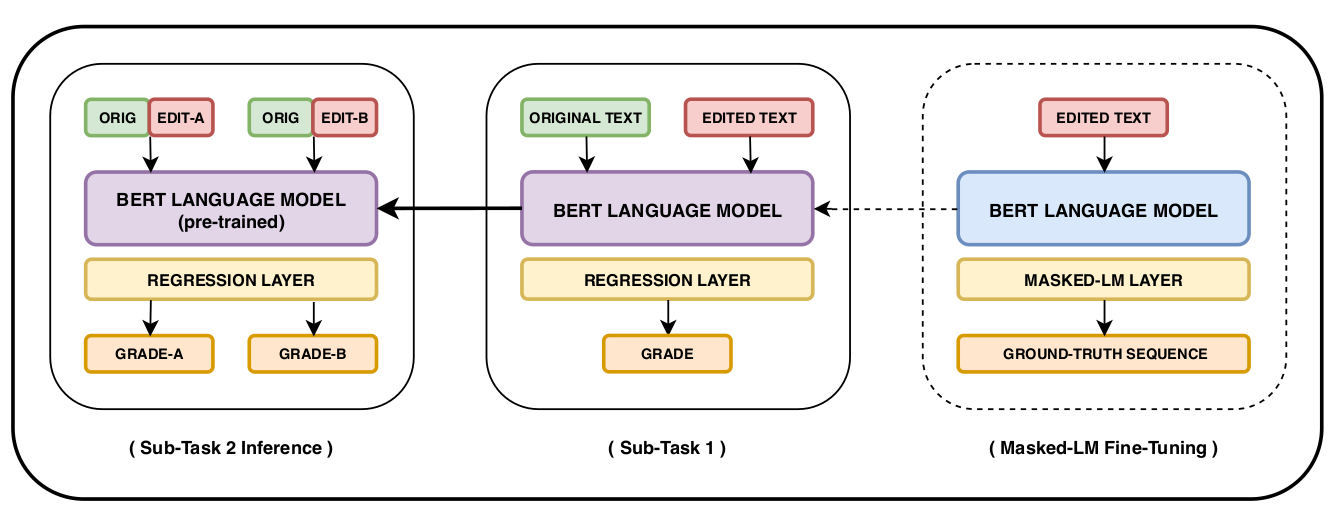
\includegraphics[width=1.0\linewidth]{system_architecture.png}

			\end{center}
			
			\caption{ Taken from \cite{Bert1} }\label{fig1}
		\end{figure}
		


	\section{Method}
		We have access to the humicroedit data set and an additional funlines data set (\textcite{Bert2} ).
		For our approach we only used the humicroedit data set and split the data in 64\%(train) to 16\%(validation) to 20\% (test) fashion. The data is split into 10 columns although for us the most relevant are the following: original1, edit1, meanGrade1, original2, edit2, meanGrade2, label.
		The original1 and original2 are the same headline but only differ by the word which gets replaced while edit1 and edit2 are two different entities which will replace those words in original1 and original2. The label tells us which edited headline is funnier by using the meanGrade1 and meanGrade2 column.
		In this section we use a different approach: similar to the approach mentioned in the related work section we concatenated original headlines with edited headlines but instead of generating 2 sentences we concatenate them again to one sentence in following manner: original1 + edited1 + original2 + edited2.
		This new sentence is fed as input into our model which is shown in figure 3.
		Our model differs from the usual approach seen in the competition(regression task for task 1 and task 2), instead we try a multi class classification approach with 3 classes. Namely 0, 1, 2 with the meaning "0": both edited headlines are equally funny, "1" first headline is funnier than second and "2" second headline is funnier than first.
		We chose a sequence length of 256, a batch size of 8 for all our data sets (train, dev, test) with two input layers for the input ids and the attention mask.
		Between the BERT layer and our final output layer we put a Dense layer of size 1024 for better generalization which gave slightly better results. 
		Finally we added a last output layer with a softmax activation function over 3 output classes.
		As optimizer we chose Adam with a learning rate of 0.00001 and a decay of 0.00000001. As loss function we chose the categorical crossentropy. We used the tensorflow implementation for the pretrained BERT model (www.huggingface.co) which is quiet large in size compared to other models.
		\pagebreak
	\begin{figure}[htb!]
		\begin{center}
		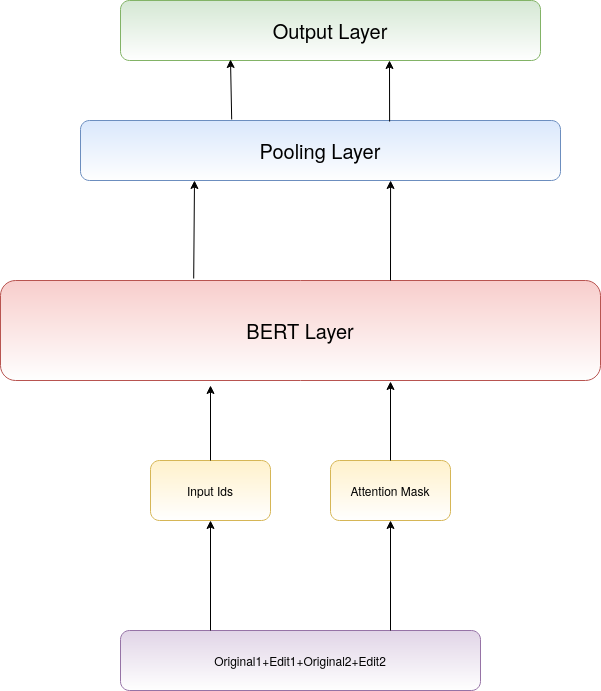
\includegraphics[width=0.5\linewidth]{My_Model_Architecture.png}
			
		\end{center}
		
		\caption{My Model Architecture}\label{fig2}
	\end{figure}
		


		
	\section{Evaluation}
    In this section we want to see how our own model and approach fares against the other participants in the competition especially against the model by \textcite{Bert1} using the pretrained BERT model .
    We tested our approach with 3 different sizes of the BERT model namely bert-base-cased, bert-base-uncased, bert-large-uncased and evaluated those models on our test set. In the competition accuracy is mostly used for evaluating sub task 2. See \textcite{Bert2}
    As we can see in Table \ref{fig3} and in Figure \ref{tab2} that our results are worse than \textcite{Bert1} and in comparison to other regression based solutions for sub task 2.
		
		
	\begin{figure}[htb!]
	\begin{center}
		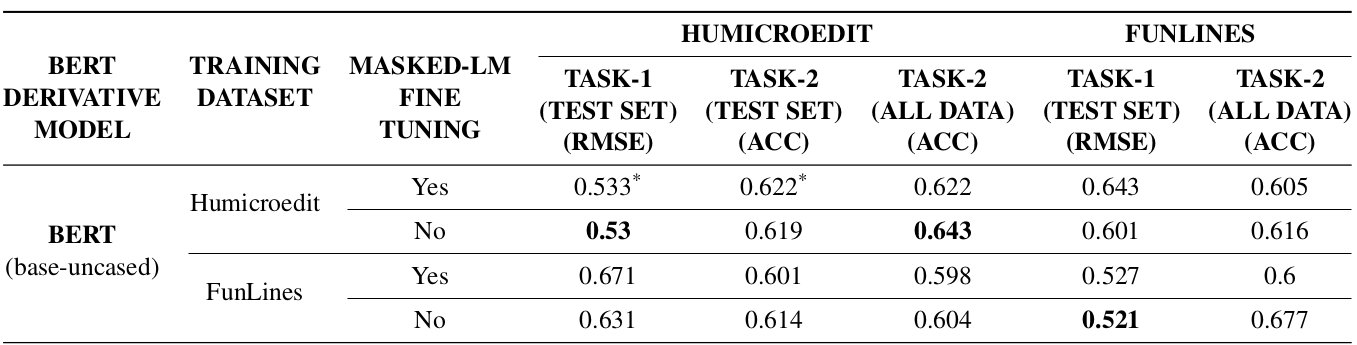
\includegraphics[width=1.0\linewidth]{eval_tab_edited2.png}
		
	\end{center}
	
	\caption{Evaluation scores taken from \textcite{Bert1}}\label{tab2}
\end{figure}


    

\begin{table}
	\begin{center}
	\begin{tabular}{|c|c|}
		\hline
		\textbf{Model} &  \textbf{Accuracy}\\
		\hline
		\hline
		BERT base cased & \textbf{0.45}\\
		\hline
		BERT base uncased & \textbf{0.48}\\
		\hline
		BERT large uncased & \textbf{0.46}\\
		\hline
	\end{tabular}
	
	
	\caption{Results}\label{fig3}
	\end{center}
	
\end{table}		
\pagebreak
	\section{Conclusion}
	In this work we tested the ability of the pretrained BERT Model for state of the art NLP tasks to be precise assessing humor in edited headlines. With little effort one can achieve relatively good results on a custom fine tuned model.  Almost every competitor used their model architecture from sub task 1 and used it for sub task 2. Those who didn't choose this approach had significantly lower results(\textcite{Bert2}). Also picking the right pretrained model had quite an influence on the results . Score wise we can see that RoBERTa seems to be leading closely followed by BERT. We have seen that state of the art approaches  only achieve mediocre results compared to other NLP tasks (Rank 1 : Team Hitachi on RoBERTa, task 1: RMSE: 0.522 , task 2: Accuracy: 0.65) (\textcite{Bert2}). This shows humor related NLP tasks still need a lot more research and work done.
	Future work could include experimenting with different pretrained models, trying new language model techniques or different approaches in customizing the input. We could also use a regression based approach for our sub task since it gave better results.
	\printbibliography
\end{document}